\حصہ{اضافی شرح نمو}
اس حصہ میں \عددی{x} کی بڑھتی قیمت پر \عددی{x} کے تفاعل کی شرح تبدیلی پر غور کیا جائے گا۔ ہم ان تفاعل پر غور کریں گے جو \عددی{x\to \infty} کرنے سے آخر کار مثبت ہو کر مثبت ہی رہتے ہیں۔ 

\جزوحصہء{اضافی شرح نمو}
آپ نے دیکھا ہو گا کہ  متغیر  \عددی{x} بڑھانے سے کثیر رکنی اور ناطق تفاعل (جنہیں ہم نے باب \حوالہ{باب_تفرق_کا_استعمال} میں ترسیم کیا تھا) کے لحاظ سے قوت نما تفاعل، مثلاً \عددی{2^x} اور \عددی{e^x}، زیادہ تیزی سے بڑھتے ہیں۔ قوت نما تفاعل یقیناً \عددی{x} کے لحاظ سے زیادہ تیزی سے بڑھتے ہیں۔ آپ شکل \حوالہ{شکل_ماورائی_قوت_نما_اور_دیگر_تفاعل} میں دیکھ سکتے ہیں کہ \عددی{x}بڑھانے سے \عددی{x^2} کے لحاظ سے  \عددی{2^x} زیادہ تیزی سے بڑھتا ہے۔ درحقیقت \عددی{x\to \infty} کرنے سے تفاعل \عددی{2^x} اور \عددی{e^x} کے بڑھنے کی شرح، \عددی{x} کے کسی بھی طاقت (مثلاً \عددی{x^{\num{1000000}}}) کے بڑھنے کی شرح سے زیادہ ہو گی۔
\begin{figure}
\centering
\begin{minipage}{0.45\textwidth}
\centering
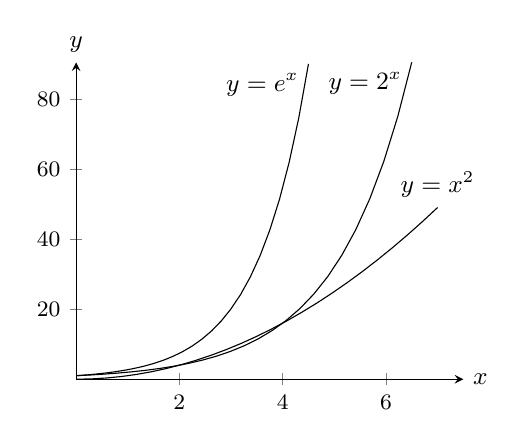
\begin{tikzpicture}[font=\small]
\begin{axis}[clip=false,small,axis lines=middle,xmin=0,ymin=0,xlabel={$x$},ylabel={$y$},xlabel style={at={(current axis.right of origin)},anchor=west},ylabel style={at={(current axis.above origin)},anchor=south},xmax=7.5]
\addplot[domain=0:4.5]{e^x}node[below left]{$y=e^x$};
\addplot[domain=0:6.5]{2^x}node[below left]{$y=2^x$};
\addplot[domain=0:7]{x^2}node[above]{$y=x^2$};
\end{axis}
\end{tikzpicture}
\caption{
تفاعل \عددی{y=e^x}، \عددی{y=2^x} اور تفاعل \عددی{y=x^2}
}
\label{شکل_ماورائی_قوت_نما_اور_دیگر_تفاعل}
\end{minipage}\hfill
\begin{minipage}{0.45\textwidth}
\centering
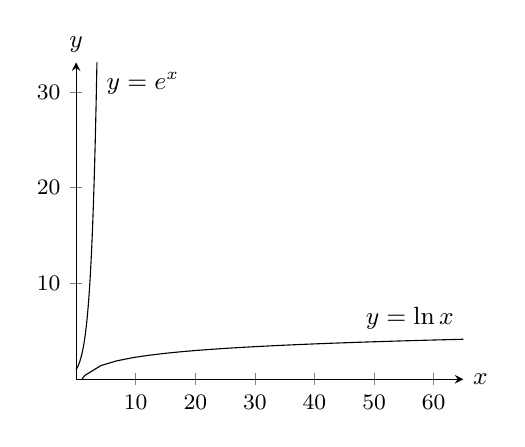
\begin{tikzpicture}[font=\small]
\begin{axis}[clip=false,small,axis lines=middle,xmin=0,ymin=0,xlabel={$x$},ylabel={$y$},xlabel style={at={(current axis.right of origin)},anchor=west},ylabel style={at={(current axis.above origin)},anchor=south}]
\addplot[domain=0:3.5]{e^x}node[below right]{$y=e^x$};
\addplot[domain=1:1.5]{ln(x)};
\addplot[domain=1.5:65]{ln(x)}node[above left]{$y=\ln x$};
\end{axis}
\end{tikzpicture}
\caption{
تفاعل \عددی{y=e^x} اور \عددی{y=\ln x} کا موازنہ
}
\label{شکل_ماورائی_قوت_نما_اور_لوگارتھمی_تفاعل}
\end{minipage}
\end{figure}

متغیر \عددی{x} بڑھاتے ہوئے تفاعل \عددی{y=e^x} کے بڑھنے کی شرح کو سمجھنے کی خاطر تصور کریں کہ آپ اس تفاعل کو ترسیم کرتے ہیں جہاں محور کا پیمانہ  \عددی{\SI{1}{\centi\meter}} ہے۔یوں \عددی{x=\SI{1}{\centi\meter}} پر \عددی{y=e^1\approx \SI{3}{\centi\meter}} ہو گا۔ یوں \عددی{x=\SI{6}{\centi\meter}} پر \عددی{y=e^6\approx\SI{403}{\centi\meter}} یعنی تقریباً \عددی{4} میٹر ہو گا جو کمرے کی چھت کے برابر ہو گا۔اسی طرح \عددی{x=\SI{10}{\centi\meter}} پر
 \عددی{y=e^{10}\approx \SI{22026}{\centi\meter}} یعنی \عددی{\SI{220}{\meter}} ہو گا جو شہر کے عموماً عمارتوں سے زیادہ بلند ہو گا۔ اگر \عددی{x=\SI{24}{\centi\meter}} ہو تب \عددی{y} چاند تک آدھے فاصلہ سے زیادہ طے کر چکا ہو گا اور \عددی{x=\SI{24}{\centi\meter}} پر \عددی{y} سورج کے قریب ترین ستارہ سے زیادہ دور ہو گا:
\begin{align*}
e^{43}&\approx \SI{4.73e18}{\centi\meter}\\
&=\SI{4.73e13}{\kilo\meter}\\
&\approx \text{\RL{$5$ نوری سال}}
\end{align*} 
اس کے باوجود \عددی{x} محور پر آپ مبدا سے صرف \عددی{\SI{43}{\centi\meter}} فاصلہ پر ہوں گے۔

اس کے برعکس \عددی{x\to\infty} کرنے سے لوگارتھمی تفاعل \عددی{y=\log_2x} اور \عددی{y=\ln x} کے بڑھنے کی شرح \عددی{x} کے کسی بھی مثبت طاقت کے بڑھنے کی شرح سے کم ہو گا۔یوں محور کا پیمانہ \عددی{\SI{1}{\centi\meter}} لیتے ہوئے مبدا سے صرف \عددی{\SI{43}{\centi\meter}} بلندی تک پہنچنے کی خاطر آپ کو محور \عددی{x} پر \عددی{5} نوری سال دور جانا ہو گا (شکل \حوالہ{شکل_ماورائی_قوت_نما_اور_لوگارتھمی_تفاعل})۔

قوت نما، کثیر رکنی اور لوگارتھمی تفاعل کا ایک دوسرے کے ساتھ مذکورہ بالا موازنہ کو زیادہ درستگی سے بیان کرنے کی خاطر ہم ایک تعریف پیش کرتے ہیں۔جب ہم کہتے ہیں کہ \عددی{x\to \infty} کرنے سے کسی بھی تفاعل \عددی{g(x)} کے بڑھنے کی شرح سے  تفاعل \عددی{f(x)} کے بڑھنے کی شرح زیادہ ہے تب اس سے مراد درج ذیل ہو گا۔

\ابتدا{تعریف}\موٹا{\عددی{x\to \infty} کرتے ہوئے بڑھنے کی شرح}\\
فرض کریں کافی بڑے \عددی{x} کے لئے \عددی{f(x)} اور \عددی{g(x)} مثبت ہیں۔
\begin{enumerate}[a.]
\item
اگر 
\begin{align*}
\lim_{x\to\infty}\frac{f(x)}{g(x)}=\infty
\end{align*}
یا، اس کا مماثل
\begin{align*}
\lim_{x\to\infty}\frac{g(x)}{f(x)}=0
\end{align*}

ہو تب  \عددی{x\to\infty} کرتے ہوئے \عددی{f} کے بڑھنے کی شرح، \عددی{g} کے بڑھنے کی شرح سے زیادہ ہو گی۔ ہم یہ بھی کہہ سکتے ہیں کہ \عددی{x\to\infty} کرتے ہوئے \عددی{g} کے بڑھنے کی شرح، \عددی{f} کے بڑھنے کی شرح سے کم ہو گی۔
\item
اگر
\begin{align*}
\lim_{x\to\infty}\frac{f(x)}{g(x)}&=L=\ne 0&&\text{\RL{$L$ غیر صفر اور متناہی ہے}}
\end{align*}
ہو تب \عددی{x\to \infty} کرتے ہوئے \عددی{f} کے بڑھنے کی شرح،  \عددی{g} کے بڑھنے کی شرح کے برابر ہو گی۔
\end{enumerate}
\انتہا{تعریف}
%====================

ان تعریف کے تحت  تفاعل \عددی{y=2x} تفاعل \عددی{y=x} سے زیادہ تیزی سے نہیں بڑھتا ہے۔ اس کی وجہ 
\begin{align*}
\lim_{x\to\infty}\frac{2x}{x}=\lim_{x\to \infty}2=2
\end{align*}
ہے  جو غیر صفر اور متناہی حد ہے۔ زیادہ تیزی سے بڑھنے کے عمومی مطلب کو ہم اس لئے نظر انداز  کرتے ہیں کہ جب ہم کہیں کہ \عددی{x} کی بڑی قیمتوں کے لئے \عددی{f} کے بڑھنے کی شرح \عددی{g} کے بڑھنے کی شرح سے زیادہ ہے تب اس سے مراد "\عددی{x} کی بڑی قیمتوں کے لئے \عددی{f} کے لحاظ سے \عددی{g} کی قیمت قابل نظر انداز ہے،" لینا چاہیے۔

\ابتدا{مثال}
\عددی{x\to\infty} کرتے ہوئے \عددی{x^2} کے لحاظ سے \عددی{e^x} درج ذیل کی بنا زیادہ تیزی سے بڑھتا ہے۔
\begin{align*}
\underbrace{\lim_{x\to\infty}\frac{e^x}{x^2}}_{\tfrac{\infty}{\infty}}&=
\underbrace{\lim_{x\to\infty}\frac{e^x}{2x}}_{\tfrac{\infty}{\infty}}=\lim_{x\to\infty}\frac{e^x}{2}=\infty
&&\text{\RL{قاعدہ لھوپیٹال دو مرتبہ استعمال کیا گیا}}
\end{align*}
\انتہا{مثال}
%===================
\ابتدا{مثال}
(ا) \عددی{x\to \infty} کرتے ہوئے \عددی{2^x} کے لحاظ سے \عددی{3^x} زیادہ تیزی سے بڑھتا ہے چونکہ:
\begin{align*}
\lim_{x\to \infty}\frac{3^x}{2^x}=\lim_{x\to \infty}\big(\frac{3}{2}\big)^x=\infty
\end{align*}
(ب) \عددی{x\to\infty} کرتے ہوئے مختلف اساس کے قوت نما تفاعل کبھی بھی ایک شرح شے نہیں بڑھتے ہیں۔اگر \عددی{a>b>0} ہو تب \عددی{a^x} کے بڑھنے کی شرح \عددی{b^x} کے بڑھنے کی شرح سے زیادہ ہو گی۔
\begin{align*}
\lim_{x\to\infty}\frac{a^x}{b^x}=\lim_{x\to\infty}\big(\frac{a}{b}\big)^x=\infty
\end{align*}
\انتہا{مثال}
%=============
\ابتدا{مثال}
\عددی{x\to\infty} کرتے ہوئے \عددی{x^2} کے بڑھنے کی شرح \عددی{\ln x} کے بڑھنے کی شرح سے زیادہ ہو گی:
\begin{align*}
\lim_{x\to\infty}\frac{2^x}{\ln x}=\lim_{x\to \infty}\frac{2x}{1/x}=\lim_{x\to\infty}2x^2=\infty
\end{align*}
\انتہا{مثال}
%================
\ابتدا{مثال}
\عددی{x\to\infty} کرنے سے \عددی{\ln x} کے بڑھنے کی شرح \عددی{x} کے بڑھنے کی شرح سے کم ہو گی:
\begin{align*}
\lim{x\to\infty}\frac{\ln x}{x}=\lim_{x\to \infty}\frac{1/x}{1}=\lim_{x\to\infty}\frac{1}{x}=0
\end{align*} 
\انتہا{مثال}
%================
\ابتدا{مثال}
قوت نما تفاعل کے برعکس \عددی{x\to\infty} کرتے ہوئے مختلف اساس کے لوگارتھمی تفاعل ایک جیسے شرح سے بڑھتے  ہیں:
\begin{align*}
\lim{x\to\infty}\frac{\log_a x}{\log_b x}=\lim_{x\to\infty}\frac{\ln x/\ln a}{\ln x/\ln b}=\frac{\ln b}{\ln a}
\end{align*} 
یہ حد غیر صفر اور متناہی ہے۔
\انتہا{مثال}
%======================

اگر \عددی{x\to\infty} کرتے ہوئے \عددی{f} کے بڑھنے کی شرح اور \عددی{g} کے بڑھنے کی شرح ایک دوسرے کے برابر ہو، اور \عددی{x\to\infty} کرتے ہوئے \عددی{gf} کے بڑھنے کی شرح اور \عددی{h} کے بڑھنے کی شرح ایک دوسرے کے برابر ہو، تب \عددی{x\to \infty} کرتے ہوئے \عددی{f} اور \عددی{h} کے بڑھنے کی شرح ایک دوسرے کے برابر ہو گی۔ اس کی وجہ
\begin{align*}
\lim_{x\to \infty}\frac{f}{g}=L_1\quad \text{اور}\quad \lim_{x\to\infty}\frac{g}{h}=L_2
\end{align*}
یعنی
\begin{align*}
\lim_{x\to\infty}\frac{f}{h}=\lim_{x\to\infty}\frac{f}{g}\cdot\frac{g}{h}=L_1L_2
\end{align*}
ہے۔اگر \عددی{L_1} اور \عددی{L_2} غیر صفر اور متناہی ہوں تب \عددی{L_1L_2} بھی غیر صفر اور متناہی ہو گا۔

\ابتدا{مثال}
دکھائیں کہ \عددی{x\to\infty} کرتے ہوئے \عددی{\sqrt{x^2+5}} اور \عددی{(2\sqrt{x}-1)^2} کے بڑھنے کی شرح ایک دوسرے جتنی ہے۔

حل:\quad
ہم دکھاتے ہیں کہ دونوں تفاعل کے بڑھنے کی شرح رہی ہے جو تفاعل \عددی{x} کی ہے:
\begin{align*}
\lim_{x\to\infty}\frac{\sqrt{x+5}}{x}&=\lim_{x\to\infty}\sqrt{1+\frac{5}{x^2}}=1\\
\lim_{x\to\infty}\frac{(2\sqrt{x}-1)^2}{x}&=\lim_{x\to \infty}\big(\frac{2\sqrt{x}-1}{\sqrt{x}}\big)^2=\lim_{x\to\infty}\big(2-\frac{1}{\sqrt{x}}\big)^2=4
\end{align*}
یوں دونوں تفاعل کے بڑھنے کی شرح ایک دوسرے جتنے ہو گی۔
\انتہا{مثال}
%=======================

\جزوحصہء{رتبہ}
